\section{Experiments and results}

\subsection{Setup}

\paragraph{LLMs and capability scaling.}

Three OpenAI models form a capability ladder, measured rather than assumed
(Table~\ref{tab:tiers}). The ladder is monotone on both benchmarks and spans single-doctor
accuracy from 25\% to 55\% on MedXpertQA, straddling the 45\% threshold of
\citet{kim2026scaling} from both sides. Following their observation that a task-grounded
capability metric explains more variance than a generic intelligence index, we use each model's
single-doctor chain-of-thought accuracy on MedQA as the capability index $I$.

\begin{table}[t]\centering\small
\caption{Capability ladder, measured on 40 items per benchmark with single-doctor CoT.}
\label{tab:tiers}
\begin{tabular}{@{}lllrrr@{}}
\toprule
Tier & Model & Effort & MedXpertQA & MedQA & USD / 1k items \\
\midrule
T1 & \texttt{gpt-4.1-nano} & --- & 25.0\% & 75.0\% & 0.09 \\
T2 & \texttt{gpt-5-nano} & low & 37.5\% & 95.0\% & 0.17 \\
T3 & \texttt{gpt-5-mini} & low & 55.0\% & 97.5\% & 0.64 \\
\bottomrule
\end{tabular}
\end{table}


\paragraph{Metrics and validation.}


We measure the coordination quantities of \citet{kim2026scaling}. Where they give a metric name
and headline value but not a closed form, we state ours explicitly.

\begin{itemize}\itemsep2pt
\item \textbf{Turns} $T$: reasoning--response exchanges; one model call is one turn.
\item \textbf{Message density} $c$: peer-opinion exposures per turn. Independent has
$C = \emptyset$ and therefore $c = 0$ by construction; Centralized exposes opinions only to the
orchestrator; Decentralized and Hybrid expose every agent to every other each round.
\item \textbf{Redundancy} $R$: mean pairwise Jaccard overlap of rationale tokens among first
opinions. High $R$ means the panel is restating one another rather than contributing independent
information.
\item \textbf{Overhead} $O\%$: token cost relative to the single-agent baseline on the same items,
$(\mathrm{tok}_{\mathrm{MAS}} - \mathrm{tok}_{\mathrm{SAS}})/\mathrm{tok}_{\mathrm{SAS}}$.
\item \textbf{Coordination efficiency} $\Ec$: accuracy divided by the token-cost ratio to the
single-agent baseline.
\item \textbf{Error absorption}: $(\!E_{\mathrm{SAS}} - E_{\mathrm{MAS}})/E_{\mathrm{SAS}}$,
exactly as defined by \citet{kim2026scaling}, where $E$ is the error rate.
\item \textbf{Error amplification} $\Ae$: they describe this as individual-agent errors reaching
the final output without inter-agent verification. We measure exactly that failure --- the panel
\emph{held} the correct option among its first opinions and still emitted a wrong one ---
normalised by the marginal probability that a single agent is wrong. $\Ae > 1$ means the system
destroys information it already possessed.
\end{itemize}

\paragraph{Budget-matched controls.}

Every configuration is accompanied by three single-model controls: zero-shot, chain-of-thought,
and \textbf{self-consistency at a matched budget}. The self-consistency pool is built from cached
$n{=}8$ sampling calls (the API maximum), so any $k$ is a prefix of the same samples; nominal cost
is charged as $\lceil k/8 \rceil$ prompts plus $k$ completions, which is what an efficient
implementation would actually pay. Panels are compared against the self-consistency cell whose
mean per-item \emph{dollar} cost is closest, not the one with a matching sample count: matching on
samples silently favours the panel, because a panel pays the prompt once per agent while
self-consistency amortises it across a batch.

Cost accounting is \emph{nominal} throughout. Cached calls are charged at list price, so the
economics figures report what a configuration would cost to run, not what our cache made it cost.

\paragraph{Scaling law.}

We fit the functional form of \citet{kim2026scaling},
\begin{align}
P = \beta_0 &+ \beta_1 I + \beta_2 I^2 + \beta_3 \log(1{+}T_{\text{tools}}) + \beta_4 \log(1{+}n_a)
 + \beta_5 \log(1{+}O\%) + \beta_6 c + \beta_7 R \nonumber\\
&+ \beta_8 \Ec + \beta_9 \log(1{+}\Ae) + \beta_{10} \PSA + \textstyle\sum_j \beta_j (\text{interactions}),
\end{align}
with interactions $I{\times}\Ec$, $\Ae{\times}\PSA$, $R{\times}n_a$, $c{\times}I$ and
$\PSA{\times}\log(1{+}n_a)$. Our tasks use no tools, so $T_{\text{tools}} = 0$ identically and
every term containing it vanishes: we fit the $T{=}0$ slice, which is the point of the study.
Standard errors are clustered by benchmark; cross-validated $R^2$ is reported over five folds.

\paragraph{Statistics.}

Paired McNemar tests with exact binomial $p$-values on identical item sets, Holm-corrected within
each family of comparisons. Wilson 95\% confidence intervals for all accuracies. Power was
calibrated on a 200-item pilot: median discordance between configurations is 8.5\%, giving a
minimum detectable difference of 5.7 percentage points at $n{=}200$ and 2.6 points at $n{=}1000$
with 80\% power. Configurations that fail for infrastructure reasons (rate limits, timeouts) are
recorded with an error status and excluded from accuracy; they are never scored as wrong answers,
which would bias call-heavy architectures downward.



\begin{figure}[t]\centering
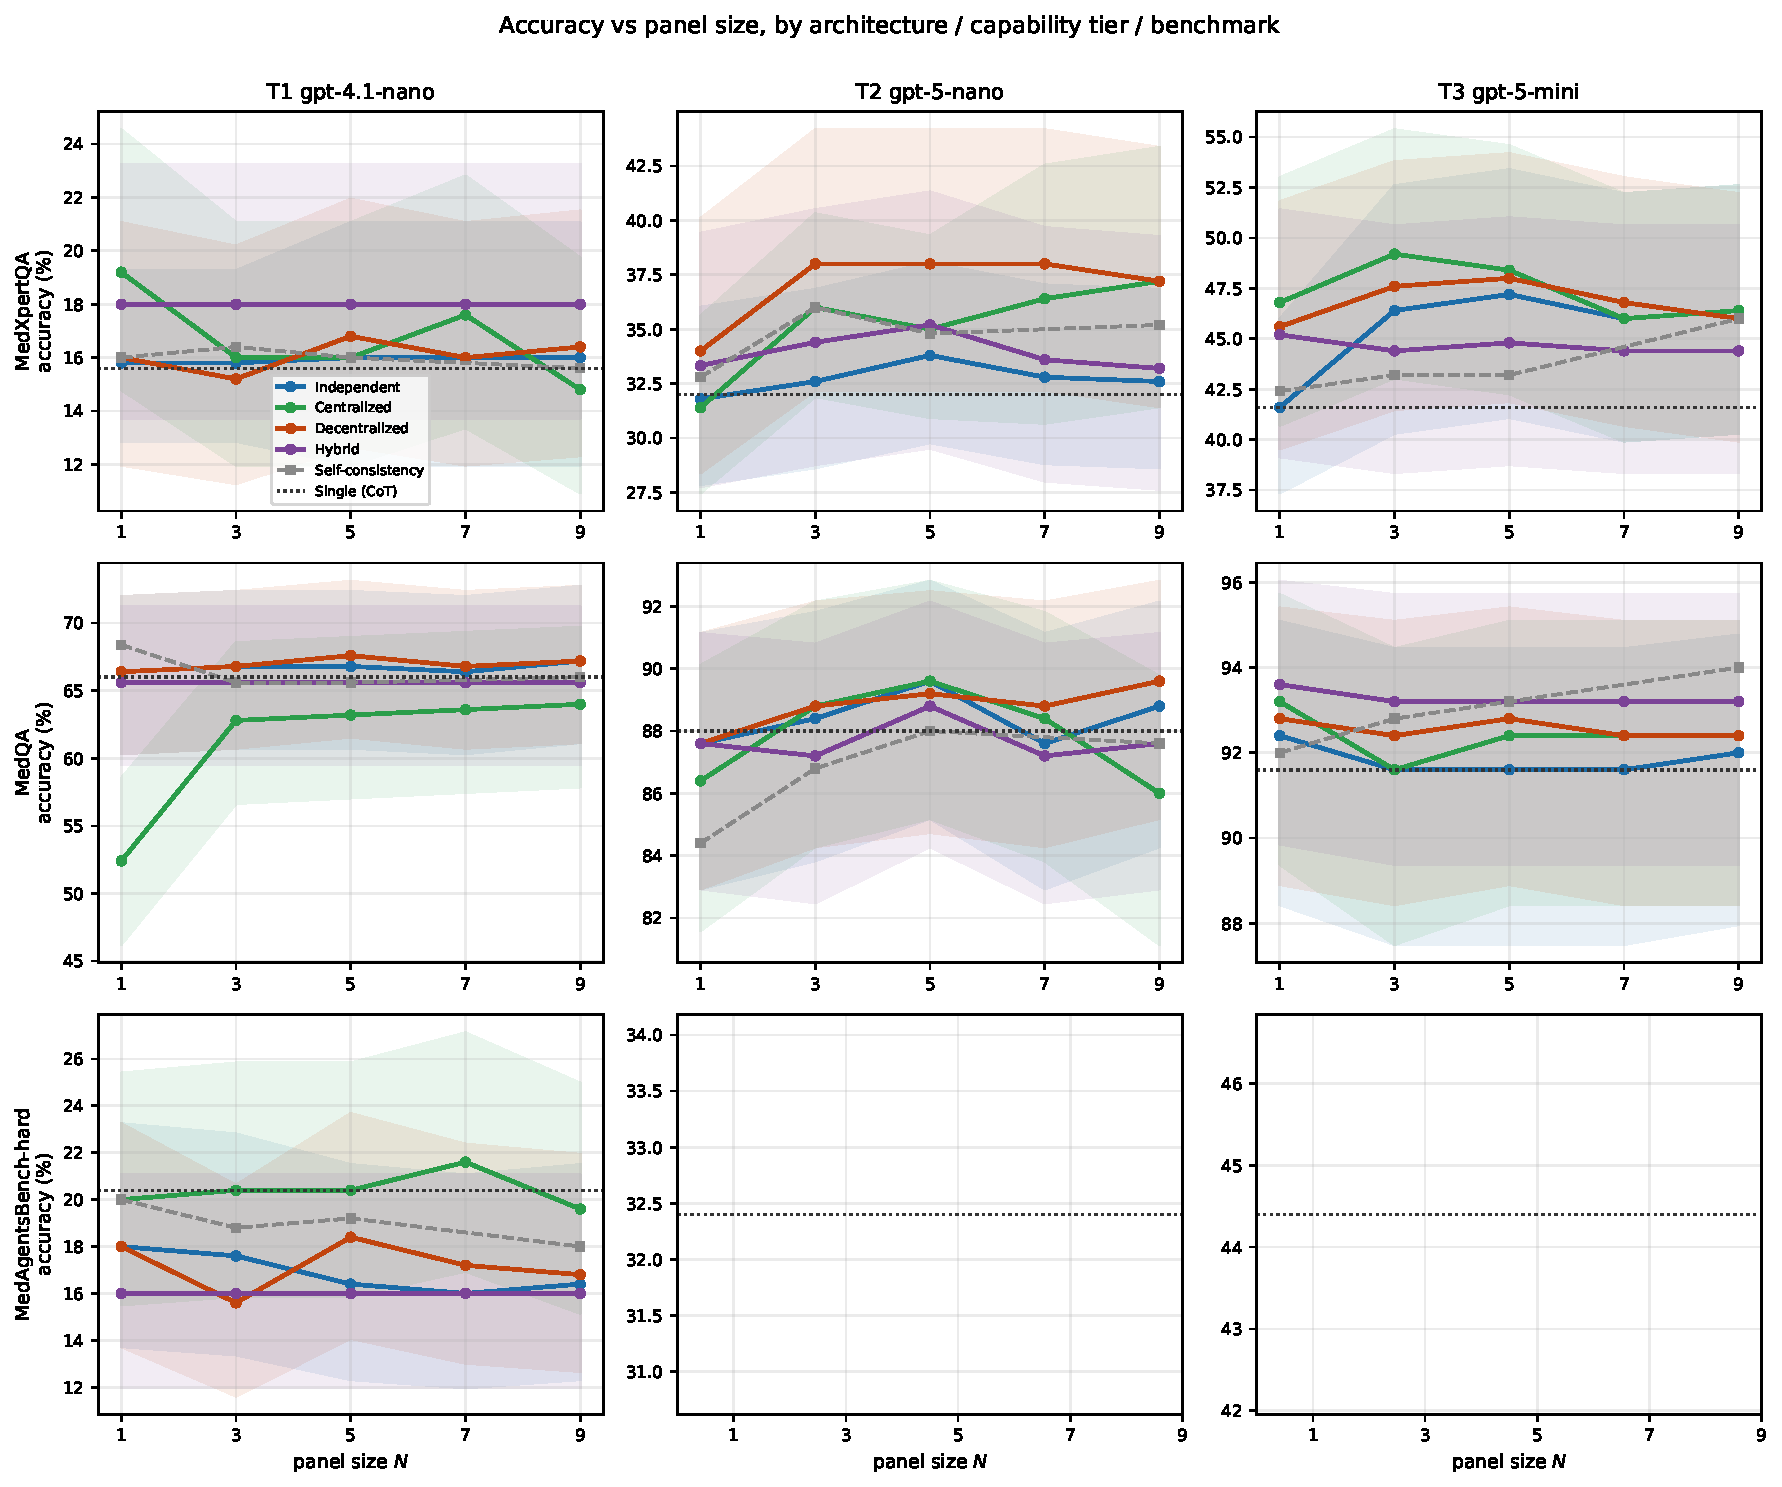
\includegraphics[width=\textwidth]{figures/fig1_curves.pdf}
\caption{Accuracy versus panel size $N$, for each architecture (colour), capability tier (column)
and benchmark (row). Bands are Wilson 95\% CIs. Dotted line: single doctor with chain-of-thought.
Dashed grey: budget-matched self-consistency. Gains, where they exist, saturate by $N{=}3$.}
\label{fig:curves}
\end{figure}

\begin{figure}[t]\centering
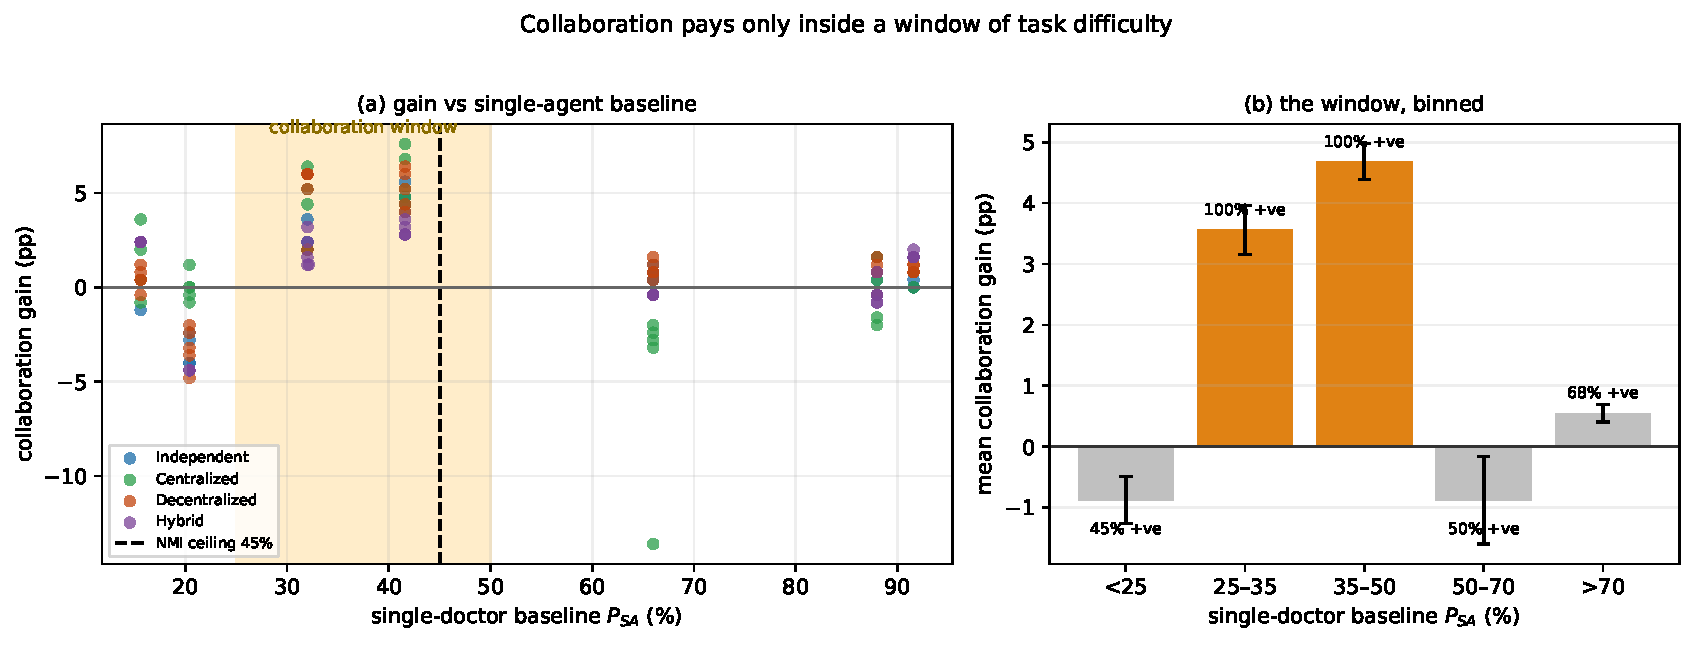
\includegraphics[width=\textwidth]{figures/fig3_threshold.pdf}
\caption{\textbf{Collaboration pays only inside a window of task difficulty.} (a) Collaboration
gain against the single-doctor baseline $\PSA$ for all 140 multi-agent configurations; shaded band
marks the 25--50\% window, dashed line the 45\% ceiling reported for general-domain agent systems
\citep{kim2026scaling}. (b) The same data binned, with the fraction of configurations showing a
positive gain. Every configuration inside the window improves on the single doctor.}
\label{fig:threshold}
\end{figure}

\begin{figure}[t]\centering
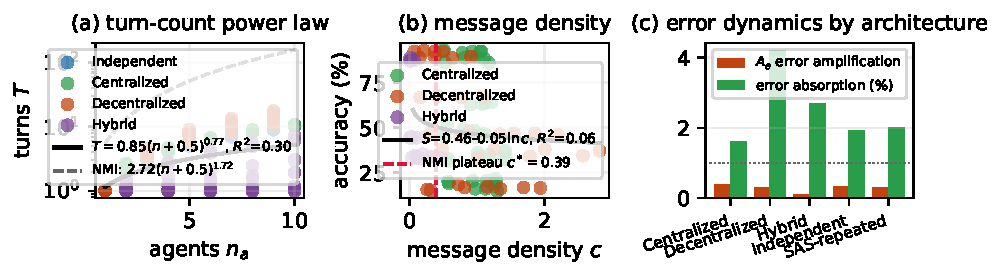
\includegraphics[width=\textwidth]{figures/fig4_coordination.pdf}
\caption{Coordination dynamics. (a) Turn count against agent count, with our fit and the
general-domain power law. (b) Accuracy against message density; the $c^{*}=0.39$ plateau of
\citet{kim2026scaling} is marked. (c) Error amplification $\Ae$ and error absorption by
architecture class.}
\label{fig:coord}
\end{figure}

\begin{figure}[t]\centering
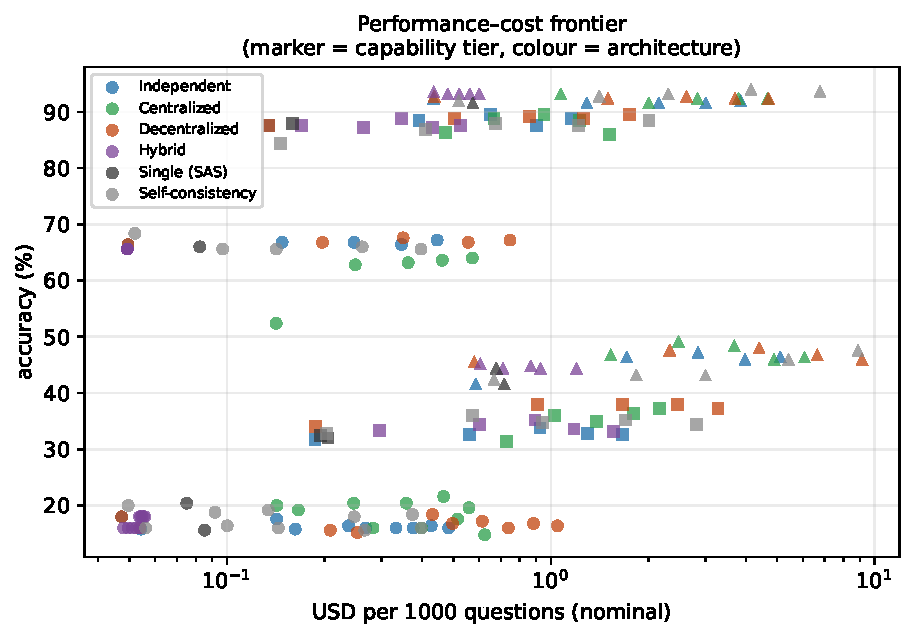
\includegraphics[width=0.72\textwidth]{figures/fig2_cost.pdf}
\caption{Performance--cost frontier. Marker shape is capability tier, colour is architecture.
Cost is nominal USD per 1{,}000 questions at list prices.}
\label{fig:cost}
\end{figure}

\begin{table}[t]\centering\scriptsize
\caption{Main results: accuracy by tier, benchmark, architecture and panel size.}
\label{tab:main}
\begin{tabular}{@{}llrrrr@{}}
\toprule
Tier & Architecture & $N$ & Accuracy (\%) & 95\% CI & USD/1k \\
\midrule
\multicolumn{6}{@{}l}{\textit{MedAgentsBench-hard}} \\
T1 & Centralized & 1 & 20.0 & [15.5, 25.4] & 0.14 \\
T1 & Centralized & 3 & 20.4 & [15.9, 25.8] & 0.25 \\
T1 & Centralized & 5 & 20.4 & [15.9, 25.8] & 0.36 \\
T1 & Centralized & 7 & 21.6 & [16.9, 27.1] & 0.47 \\
T1 & Centralized & 9 & 19.6 & [15.2, 25.0] & 0.56 \\
T1 & Decentralized & 1 & 18.0 & [13.7, 23.2] & 0.05 \\
T1 & Decentralized & 3 & 15.6 & [11.6, 20.6] & 0.21 \\
T1 & Decentralized & 5 & 18.4 & [14.1, 23.7] & 0.43 \\
T1 & Decentralized & 7 & 17.2 & [13.0, 22.4] & 0.61 \\
T1 & Decentralized & 9 & 16.8 & [12.7, 21.9] & 0.88 \\
T1 & Hybrid & 1 & 16.0 & [12.0, 21.1] & 0.05 \\
T1 & Hybrid & 3 & 16.0 & [12.0, 21.1] & 0.05 \\
T1 & Hybrid & 5 & 16.0 & [12.0, 21.1] & 0.05 \\
T1 & Hybrid & 7 & 16.0 & [12.0, 21.1] & 0.05 \\
T1 & Hybrid & 9 & 16.0 & [12.0, 21.1] & 0.05 \\
T1 & Independent & 1 & 18.0 & [13.7, 23.2] & 0.05 \\
T1 & Independent & 3 & 17.6 & [13.4, 22.8] & 0.14 \\
T1 & Independent & 5 & 16.4 & [12.3, 21.5] & 0.24 \\
T1 & Independent & 7 & 16.0 & [12.0, 21.1] & 0.33 \\
T1 & Independent & 9 & 16.4 & [12.3, 21.5] & 0.43 \\
T1 & SAS CoT & 1 & 20.4 & [15.9, 25.8] & 0.08 \\
T1 & SAS zero-shot & 1 & 16.8 & [12.7, 21.9] & 0.03 \\
T1 & Self-consistency & 1 & 20.0 & [15.5, 25.4] & 0.05 \\
T1 & Self-consistency & 3 & 18.8 & [14.4, 24.1] & 0.09 \\
T1 & Self-consistency & 5 & 19.2 & [14.8, 24.5] & 0.13 \\
T1 & Self-consistency & 9 & 18.0 & [13.7, 23.2] & 0.25 \\
T1 & Self-consistency & 15 & 18.4 & [14.1, 23.7] & 0.37 \\
T2 & SAS CoT & 1 & 32.4 & [26.9, 38.4] & 0.19 \\
\midrule
\multicolumn{6}{@{}l}{\textit{MedQA}} \\
T1 & Centralized & 1 & 52.4 & [46.2, 58.5] & 0.14 \\
T1 & Centralized & 3 & 62.8 & [56.7, 68.6] & 0.25 \\
T1 & Centralized & 5 & 63.2 & [57.1, 68.9] & 0.36 \\
T1 & Centralized & 7 & 63.6 & [57.5, 69.3] & 0.46 \\
T1 & Centralized & 9 & 64.0 & [57.9, 69.7] & 0.57 \\
T1 & Decentralized & 1 & 66.4 & [60.3, 72.0] & 0.05 \\
T1 & Decentralized & 3 & 66.8 & [60.7, 72.3] & 0.20 \\
T1 & Decentralized & 5 & 67.6 & [61.6, 73.1] & 0.35 \\
T1 & Decentralized & 7 & 66.8 & [60.7, 72.3] & 0.56 \\
T1 & Decentralized & 9 & 67.2 & [61.2, 72.7] & 0.75 \\
T1 & Hybrid & 1 & 65.6 & [59.5, 71.2] & 0.05 \\
T1 & Hybrid & 3 & 65.6 & [59.5, 71.2] & 0.05 \\
T1 & Hybrid & 5 & 65.6 & [59.5, 71.2] & 0.05 \\
T1 & Hybrid & 7 & 65.6 & [59.5, 71.2] & 0.05 \\
T1 & Hybrid & 9 & 65.6 & [59.5, 71.2] & 0.05 \\
T1 & Independent & 1 & 66.4 & [60.3, 72.0] & 0.05 \\
T1 & Independent & 3 & 66.8 & [60.7, 72.3] & 0.15 \\
T1 & Independent & 5 & 66.8 & [60.7, 72.3] & 0.25 \\
T1 & Independent & 7 & 66.4 & [60.3, 72.0] & 0.35 \\
T1 & Independent & 9 & 67.2 & [61.2, 72.7] & 0.45 \\
T1 & SAS CoT & 1 & 66.0 & [59.9, 71.6] & 0.08 \\
T1 & SAS zero-shot & 1 & 66.4 & [60.3, 72.0] & 0.03 \\
T1 & Self-consistency & 1 & 68.4 & [62.4, 73.8] & 0.05 \\
T1 & Self-consistency & 3 & 65.6 & [59.5, 71.2] & 0.10 \\
T1 & Self-consistency & 5 & 65.6 & [59.5, 71.2] & 0.14 \\
T1 & Self-consistency & 9 & 66.0 & [59.9, 71.6] & 0.26 \\
T1 & Self-consistency & 15 & 65.6 & [59.5, 71.2] & 0.40 \\
T2 & Centralized & 1 & 86.4 & [81.6, 90.1] & 0.47 \\
T2 & Centralized & 3 & 88.8 & [84.3, 92.1] & 0.67 \\
T2 & Centralized & 5 & 89.6 & [85.2, 92.8] & 0.95 \\
T2 & Centralized & 7 & 88.4 & [83.8, 91.8] & 1.23 \\
T2 & Centralized & 9 & 86.0 & [81.2, 89.8] & 1.51 \\
T2 & Decentralized & 1 & 87.6 & [82.9, 91.1] & 0.13 \\
T2 & Decentralized & 3 & 88.8 & [84.3, 92.1] & 0.50 \\
T2 & Decentralized & 5 & 89.2 & [84.7, 92.5] & 0.86 \\
T2 & Decentralized & 7 & 88.8 & [84.3, 92.1] & 1.26 \\
T2 & Decentralized & 9 & 89.6 & [85.2, 92.8] & 1.75 \\
T2 & Hybrid & 1 & 87.6 & [82.9, 91.1] & 0.17 \\
T2 & Hybrid & 3 & 87.2 & [82.5, 90.8] & 0.26 \\
T2 & Hybrid & 5 & 88.8 & [84.3, 92.1] & 0.35 \\
T2 & Hybrid & 7 & 87.2 & [82.5, 90.8] & 0.43 \\
T2 & Hybrid & 9 & 87.6 & [82.9, 91.1] & 0.53 \\
T2 & Independent & 1 & 87.6 & [82.9, 91.1] & 0.13 \\
T2 & Independent & 3 & 88.4 & [83.8, 91.8] & 0.39 \\
T2 & Independent & 5 & 89.6 & [85.2, 92.8] & 0.65 \\
T2 & Independent & 7 & 87.6 & [82.9, 91.1] & 0.90 \\
T2 & Independent & 9 & 88.8 & [84.3, 92.1] & 1.16 \\
T2 & SAS CoT & 1 & 88.0 & [83.4, 91.5] & 0.16 \\
T2 & SAS zero-shot & 1 & 87.2 & [82.5, 90.8] & 0.09 \\
T2 & Self-consistency & 1 & 84.4 & [79.4, 88.4] & 0.15 \\
T2 & Self-consistency & 3 & 86.8 & [82.0, 90.4] & 0.41 \\
T2 & Self-consistency & 5 & 88.0 & [83.4, 91.5] & 0.67 \\
T2 & Self-consistency & 9 & 87.6 & [82.9, 91.1] & 1.21 \\
T2 & Self-consistency & 15 & 88.4 & [83.8, 91.8] & 2.01 \\
T3 & Centralized & 1 & 93.2 & [89.4, 95.7] & 1.07 \\
T3 & Centralized & 3 & 91.6 & [87.5, 94.4] & 2.00 \\
T3 & Centralized & 5 & 92.4 & [88.4, 95.1] & 2.84 \\
T3 & Centralized & 7 & 92.4 & [88.4, 95.1] & 3.80 \\
T3 & Centralized & 9 & 92.4 & [88.4, 95.1] & 4.66 \\
T3 & Decentralized & 1 & 92.8 & [88.9, 95.4] & 0.44 \\
T3 & Decentralized & 3 & 92.4 & [88.4, 95.1] & 1.50 \\
T3 & Decentralized & 5 & 92.8 & [88.9, 95.4] & 2.62 \\
T3 & Decentralized & 7 & 92.4 & [88.4, 95.1] & 3.70 \\
T3 & Decentralized & 9 & 92.4 & [88.4, 95.1] & 4.70 \\
T3 & Hybrid & 1 & 93.6 & [89.9, 96.0] & 0.43 \\
T3 & Hybrid & 3 & 93.2 & [89.4, 95.7] & 0.48 \\
T3 & Hybrid & 5 & 93.2 & [89.4, 95.7] & 0.52 \\
T3 & Hybrid & 7 & 93.2 & [89.4, 95.7] & 0.56 \\
T3 & Hybrid & 9 & 93.2 & [89.4, 95.7] & 0.60 \\
T3 & Independent & 1 & 92.4 & [88.4, 95.1] & 0.43 \\
T3 & Independent & 3 & 91.6 & [87.5, 94.4] & 1.29 \\
T3 & Independent & 5 & 91.6 & [87.5, 94.4] & 2.15 \\
T3 & Independent & 7 & 91.6 & [87.5, 94.4] & 3.01 \\
T3 & Independent & 9 & 92.0 & [88.0, 94.8] & 3.86 \\
T3 & SAS CoT & 1 & 91.6 & [87.5, 94.4] & 0.57 \\
T3 & SAS zero-shot & 1 & 94.4 & [90.8, 96.6] & 0.27 \\
T3 & Self-consistency & 1 & 92.0 & [88.0, 94.8] & 0.52 \\
T3 & Self-consistency & 3 & 92.8 & [88.9, 95.4] & 1.41 \\
T3 & Self-consistency & 5 & 93.2 & [89.4, 95.7] & 2.30 \\
T3 & Self-consistency & 9 & 94.0 & [90.3, 96.3] & 4.15 \\
T3 & Self-consistency & 15 & 93.6 & [89.9, 96.0] & 6.78 \\
\midrule
\multicolumn{6}{@{}l}{\textit{MedXpertQA}} \\
T1 & Centralized & 1 & 19.2 & [14.8, 24.5] & 0.17 \\
T1 & Centralized & 3 & 16.0 & [12.0, 21.1] & 0.28 \\
T1 & Centralized & 5 & 16.0 & [12.0, 21.1] & 0.40 \\
T1 & Centralized & 7 & 17.6 & [13.4, 22.8] & 0.52 \\
T1 & Centralized & 9 & 14.8 & [10.9, 19.7] & 0.62 \\
T1 & Decentralized & 1 & 16.0 & [12.0, 21.1] & 0.05 \\
T1 & Decentralized & 3 & 15.2 & [11.3, 20.2] & 0.25 \\
T1 & Decentralized & 5 & 16.8 & [12.7, 21.9] & 0.50 \\
T1 & Decentralized & 7 & 16.0 & [12.0, 21.1] & 0.74 \\
T1 & Decentralized & 9 & 16.4 & [12.3, 21.5] & 1.05 \\
T1 & Hybrid & 1 & 18.0 & [13.7, 23.2] & 0.05 \\
T1 & Hybrid & 3 & 18.0 & [13.7, 23.2] & 0.05 \\
T1 & Hybrid & 5 & 18.0 & [13.7, 23.2] & 0.05 \\
T1 & Hybrid & 7 & 18.0 & [13.7, 23.2] & 0.06 \\
T1 & Hybrid & 9 & 18.0 & [13.7, 23.2] & 0.06 \\
T1 & Independent & 1 & 15.8 & [12.9, 19.3] & 0.05 \\
T1 & Independent & 3 & 15.8 & [12.9, 19.3] & 0.16 \\
T1 & Independent & 5 & 16.0 & [12.0, 21.1] & 0.27 \\
T1 & Independent & 7 & 16.0 & [12.0, 21.1] & 0.38 \\
T1 & Independent & 9 & 16.0 & [12.0, 21.1] & 0.48 \\
T1 & SAS CoT & 1 & 15.6 & [11.6, 20.6] & 0.09 \\
T1 & SAS zero-shot & 1 & 16.4 & [12.3, 21.5] & 0.03 \\
T1 & Self-consistency & 1 & 16.0 & [12.0, 21.1] & 0.06 \\
T1 & Self-consistency & 3 & 16.4 & [12.3, 21.5] & 0.10 \\
T1 & Self-consistency & 5 & 16.0 & [12.0, 21.1] & 0.14 \\
T1 & Self-consistency & 9 & 15.6 & [11.6, 20.6] & 0.27 \\
T1 & Self-consistency & 15 & 16.0 & [12.0, 21.1] & 0.40 \\
T2 & Centralized & 1 & 31.4 & [27.5, 35.6] & 0.73 \\
T2 & Centralized & 3 & 36.0 & [31.9, 40.3] & 1.02 \\
T2 & Centralized & 5 & 35.0 & [30.9, 39.3] & 1.38 \\
T2 & Centralized & 7 & 36.4 & [30.7, 42.5] & 1.80 \\
T2 & Centralized & 9 & 37.2 & [31.4, 43.3] & 2.17 \\
T2 & Decentralized & 1 & 34.0 & [28.4, 40.1] & 0.19 \\
T2 & Decentralized & 3 & 38.0 & [32.2, 44.2] & 0.91 \\
T2 & Decentralized & 5 & 38.0 & [32.2, 44.2] & 1.66 \\
T2 & Decentralized & 7 & 38.0 & [32.2, 44.2] & 2.46 \\
T2 & Decentralized & 9 & 37.2 & [31.4, 43.3] & 3.28 \\
T2 & Hybrid & 1 & 33.3 & [27.8, 39.4] & 0.29 \\
T2 & Hybrid & 3 & 34.4 & [28.8, 40.5] & 0.60 \\
T2 & Hybrid & 5 & 35.2 & [29.5, 41.3] & 0.89 \\
T2 & Hybrid & 7 & 33.6 & [28.0, 39.7] & 1.18 \\
T2 & Hybrid & 9 & 33.2 & [27.7, 39.3] & 1.56 \\
T2 & Independent & 1 & 31.8 & [27.9, 36.0] & 0.19 \\
T2 & Independent & 3 & 32.6 & [28.6, 36.8] & 0.56 \\
T2 & Independent & 5 & 33.8 & [29.8, 38.1] & 0.93 \\
T2 & Independent & 7 & 32.8 & [28.8, 37.0] & 1.30 \\
T2 & Independent & 9 & 32.6 & [28.6, 36.8] & 1.67 \\
T2 & SAS CoT & 1 & 32.0 & [26.5, 38.0] & 0.20 \\
T2 & SAS zero-shot & 1 & 32.4 & [26.9, 38.4] & 0.15 \\
T2 & Self-consistency & 1 & 32.8 & [27.3, 38.8] & 0.20 \\
T2 & Self-consistency & 3 & 36.0 & [30.3, 42.1] & 0.57 \\
T2 & Self-consistency & 5 & 34.8 & [29.2, 40.9] & 0.94 \\
T2 & Self-consistency & 9 & 35.2 & [29.5, 41.3] & 1.70 \\
T2 & Self-consistency & 15 & 34.4 & [28.8, 40.5] & 2.81 \\
T3 & Centralized & 1 & 46.8 & [40.7, 53.0] & 1.53 \\
T3 & Centralized & 3 & 49.2 & [43.1, 55.4] & 2.48 \\
T3 & Centralized & 5 & 48.4 & [42.3, 54.6] & 3.68 \\
T3 & Centralized & 7 & 46.0 & [39.9, 52.2] & 4.89 \\
T3 & Centralized & 9 & 46.4 & [40.3, 52.6] & 6.07 \\
T3 & Decentralized & 1 & 45.6 & [39.5, 51.8] & 0.58 \\
T3 & Decentralized & 3 & 47.6 & [41.5, 53.8] & 2.33 \\
T3 & Decentralized & 5 & 48.0 & [41.9, 54.2] & 4.39 \\
T3 & Decentralized & 7 & 46.8 & [40.7, 53.0] & 6.65 \\
T3 & Decentralized & 9 & 46.0 & [39.9, 52.2] & 9.14 \\
T3 & Hybrid & 1 & 45.2 & [39.1, 51.4] & 0.61 \\
T3 & Hybrid & 3 & 44.4 & [38.4, 50.6] & 0.71 \\
T3 & Hybrid & 5 & 44.8 & [38.8, 51.0] & 0.87 \\
T3 & Hybrid & 7 & 44.4 & [38.4, 50.6] & 0.93 \\
T3 & Hybrid & 9 & 44.4 & [38.4, 50.6] & 1.20 \\
T3 & Independent & 1 & 41.6 & [37.4, 46.0] & 0.59 \\
T3 & Independent & 3 & 46.4 & [40.3, 52.6] & 1.71 \\
T3 & Independent & 5 & 47.2 & [41.1, 53.4] & 2.84 \\
T3 & Independent & 7 & 46.0 & [39.9, 52.2] & 3.97 \\
T3 & Independent & 9 & 46.4 & [40.3, 52.6] & 5.11 \\
T3 & SAS CoT & 1 & 41.6 & [35.7, 47.8] & 0.72 \\
T3 & SAS zero-shot & 1 & 43.2 & [37.2, 49.4] & 0.46 \\
T3 & Self-consistency & 1 & 42.4 & [36.4, 48.6] & 0.67 \\
T3 & Self-consistency & 3 & 43.2 & [37.2, 49.4] & 1.83 \\
T3 & Self-consistency & 5 & 43.2 & [37.2, 49.4] & 3.00 \\
T3 & Self-consistency & 9 & 46.0 & [39.9, 52.2] & 5.41 \\
T3 & Self-consistency & 15 & 47.6 & [41.5, 53.8] & 8.87 \\
\midrule
\bottomrule
\end{tabular}
\end{table}

\subsection{Main results}

Across 175 configurations and 50{,}749 episodes we find that collaboration in medicine is
governed by task difficulty, not by panel size. Figure~\ref{fig:curves} gives the full
dose--response surface; Table~\ref{tab:main} the underlying numbers.

\paragraph{Collaboration pays only inside a window of task difficulty.}
Binning the 140 multi-agent configurations by the single-doctor baseline $\PSA$ of their cell
reveals a window rather than a ceiling (Fig.~\ref{fig:threshold}):

\begin{center}\small
\begin{tabular}{@{}lrrr@{}}
\toprule
$\PSA$ & configurations & mean gain & fraction positive \\
\midrule
$<25\%$    & 40 & $-0.88$ pp & 45\% \\
$25$--$35\%$ & 20 & $\mathbf{+3.56}$ pp & \textbf{100\%} \\
$35$--$50\%$ & 20 & $\mathbf{+4.68}$ pp & \textbf{100\%} \\
$50$--$70\%$ & 20 & $-0.88$ pp & 50\% \\
$>70\%$    & 40 & $+0.55$ pp & 68\% \\
\bottomrule
\end{tabular}
\end{center}

Every one of the 40 configurations whose baseline falls between 25\% and 50\% improves on the
single doctor. Outside that band fewer than 70\% do, and below 25\% the mean gain is negative.
Splitting at the 45\% figure of \citet{kim2026scaling} reproduces their direction --- mean gain
$+1.32$ pp below versus $+0.11$ pp above, Welch $t = 3.16$, $p = 0.0018$ --- but that split
misses half the structure. The ceiling they report is the \emph{upper} edge of a window whose
lower edge our design is able to reach, because expert-level medical items drive single-agent
accuracy down to 15\%, well below anything in their benchmark suite.

\paragraph{The window is where the significant effects live.}
Only two of the seven tier\,$\times$\,benchmark cells yield a statistically significant
collaboration gain, and both sit inside the window. On MedXpertQA the attending-physician
(Centralized) panel at $N{=}3$ gains $+7.60$ pp over the single doctor at $\PSA = 41.6\%$
(\texttt{gpt-5-mini}; McNemar $p < 10^{-4}$) and $+6.40$ pp at $\PSA = 32.0\%$
(\texttt{gpt-5-nano}; $p = 0.0037$). The five cells outside the window --- all three MedQA cells
($\PSA = 66$--$92\%$) and both cells below 25\% --- produce no significant gain from any
architecture at any panel size.

\paragraph{Architecture matters more than panel size.}
Within the window, the ordering is stable: Centralized and Decentralized lead, Hybrid trails, and
Independent voting is indistinguishable from the single doctor. On \texttt{gpt-5-nano} /
MedXpertQA, Independent moves from 31.8\% at $N{=}1$ to 32.6\% at $N{=}9$ --- 0.8 pp for nine
times the calls --- while Decentralized reaches 38.0\% at $N{=}3$ and stays there. Gains saturate
at $N{=}3$ in every cell where they occur; no architecture in any cell improves beyond $N{=}5$.

\paragraph{Architecture--capability tier interactions.}
The best architecture depends on the tier. At T2 the peak is Decentralized (38.0\%, $+6.0$ pp);
at T3 it is Centralized (49.2\%, $+7.6$ pp). This mirrors the family-dependent architectural
preferences reported by \citet{kim2026scaling}: the stronger model exploits an orchestrator's
audit, whereas the weaker model benefits more from peer exchange, whose redundancy compensates
for individually unreliable opinions.

\subsection{Scaling principles}

\paragraph{With accuracy as the response, the fit is degenerate.}
Fitting the functional form of \citet{kim2026scaling} directly gives $R^2 = 0.998$ (5-fold
cross-validated $R^2 = 0.997$), which is not a replication but an artefact of our tighter design.
Their response variable is accuracy and one predictor is $\PSA$; across six heterogeneous
benchmarks and three model families that predictor leaves ample residual variance, and they
report cross-validated $R^2 = 0.513$. In our design the same items and the same model underlie
both terms and only the coordination structure varies, so $\PSA$ alone very nearly determines
accuracy ($\hat\beta_{\PSA} = 0.880$). We therefore refit with the collaboration
\emph{gain} as the response, which is the quantity the scaling principle is actually about.

\paragraph{The gain model recovers the general-domain level of explanatory power.}
With $\mathrm{gain} = P - \PSA$ as the response, $R^2 = 0.638$ and 5-fold cross-validated
$R^2 = \mathbf{0.531}$ --- essentially the $0.513$ reported for the general-domain fit, obtained
here without any tool-count term. Coefficients ($n = 175$, benchmark-clustered SEs):

\begin{center}\small
\begin{tabular}{@{}lrrl@{}}
\toprule
term & $\hat\beta$ & $p$ & interpretation \\
\midrule
$\log(1+\Ae)$ & $-0.151$ & $<0.001$ & error amplification is the dominant penalty \\
$R$ (redundancy) & $+0.083$ & $<0.001$ & overlapping rationales help, not hurt \\
$I$ & $-2.479$ & $<0.001$ & \multirow{2}{*}{capability enters non-linearly} \\
$I^2$ & $+1.557$ & $<0.001$ & \\
$c$ (message density) & $+0.007$ & $0.011$ & communication has a small positive effect \\
$\log(1+n_a)$ & $-0.005$ & $0.673$ & \textbf{panel size does not predict gain} \\
$\PSA$ & $-0.052$ & $0.343$ & \multirow{2}{*}{no linear or quadratic $\PSA$ effect} \\
$\PSA^2$ & $-0.022$ & $0.726$ & \\
\bottomrule
\end{tabular}
\end{center}

\paragraph{The tool--coordination trade-off is absent by construction, and the capability term
survives without it.} $T_{\text{tools}} = 0$ throughout, so the $\log(1+T)$ main effect and the
$O\%\times T$ and $\Ec \times T$ interactions --- carrying $\hat\beta = -0.330$ in the
general-domain fit --- are identically zero here. The capability structure nevertheless remains
highly significant, which establishes that the capability effect is not an artefact of tool
overhead.

\paragraph{The decision boundary is not identifiable in the tool-free slice.}
\citet{kim2026scaling} derive their threshold as
$\PSA^{*} = \hat\beta_{4}/\hat\beta_{17} \approx 0.063/0.408 = 0.154$ in standardised units,
$\approx 0.45$ after denormalisation. Both ingredients are null in our fit
($\hat\beta_{\log(1+n_a)} = -0.005$, $p = 0.67$; $\hat\beta_{\PSA \times \log(1+n_a)} = +0.008$,
$p = 0.37$), so the ratio is uninterpretable. This is a finding about functional form, not a
failure to replicate: a linear interaction between baseline and log panel size cannot express a
window, and the binned analysis shows the relationship is non-monotone in $\PSA$. The
general-domain data, which never reach the difficult end, are consistent with a monotone ceiling;
the medical data are not.

\paragraph{Error amplification dominates the fit.}
$\log(1+\Ae)$ carries the largest standardised coefficient of any coordination metric
($-0.151$, $p<0.001$). $\Ae$ measures how often a panel held the correct option among its first
opinions and still emitted a wrong one. Configurations that lose information they already possess
are exactly the configurations that fail to beat the single doctor, which is the mechanism
\citet{kim2026scaling} propose from the opposite direction.

\paragraph{Redundancy provides benefit at scale.}
$R \times n_a$ is positive ($\hat\beta = +0.006$, $p = 0.040$ in the accuracy fit), reproducing
their marginal-benefit-at-scale result ($\hat\beta_{R \times n_a} = 0.041$, $p = 0.040$). In
clinical panels, specialists restating one another is a weak form of verification rather than
wasted capacity.

\subsection{Coordination efficiency, error dynamics, and information transfer}

\paragraph{Turn count does not follow the general-domain power law.}
Fitting $T = a(n+0.5)^{b}$ gives $a = 0.85$, $b = 0.752$, $R^2 = 0.282$, against
$a = 2.72$, $b = 1.724$, $R^2 = 0.974$ in the general-domain study. The exponent is sub-linear
here and super-linear there. The reason is structural: their agents negotiate open-ended tool use
with unbounded exchange, whereas a clinical panel answering a closed question terminates on
unanimity. Half of our five-expert panels are unanimous after the first round, so turns grow more
slowly than agents. The super-linear regime, and the hard resource ceiling they infer from it,
does not appear in tool-free consultation.

\paragraph{Message density does not predict accuracy.}
$S = 0.485 - 0.058\ln(c)$, $R^2 = 0.077$, against $S = 0.73 + 0.28\ln(c)$, $R^2 = 0.68$. The
plateau at $c^{*} = 0.39$ that organises their architectures does not appear: our Centralized
panels run at $c = 0.98$ and Decentralized at $c = 0.73$, both far past that point, with no
accuracy penalty. Talking more neither helps nor hurts once the panel is talking at all.

\paragraph{Error absorption is real but small.}
Absorption $(E_{\mathrm{SAS}} - E_{\mathrm{MAS}})/E_{\mathrm{SAS}}$ is positive for every
architecture: Decentralized $+4.8\%$, Hybrid $+3.1\%$, Independent $+2.2\%$, Centralized
$+1.8\%$. The general-domain study reports $22.7\%$ (95\% CI $[20.1, 25.3]$) for
verification-bearing architectures. Medical panels absorb roughly a fifth as much error as
general-domain agent teams do.

\paragraph{Error taxonomy reproduces the architecture-specific signature.}
Applying the four-category taxonomy to first-round opinions:

\begin{center}\small
\begin{tabular}{@{}lrrr@{}}
\toprule
Error category & Independent & Decentralized & \citet{kim2026scaling} \\
\midrule
Logical contradiction & 15.4\% & \textbf{11.4\%} & 16.8\% $\rightarrow$ \textbf{11.5\%} \\
Context omission & 22.2\% & 17.1\% & 24.1\% $\rightarrow$ 11.2\% \\
Numerical drift & 3.9\% & 3.1\% & 23.2\% $\rightarrow$ 18.3\% \\
Coordination failure & \textbf{0.0\%} & 1.1\% & \textbf{0\%} $\rightarrow$ present \\
\bottomrule
\end{tabular}
\end{center}

Two entries match the general-domain result almost exactly. Peer discussion reduces logical
contradiction from 15.4\% to 11.4\%, against their 16.8\% to 11.5\%. Coordination failure is
0.0\% under Independent coordination in both studies, for the same structural reason: with
$C = \emptyset$ there is no channel on which coordination can fail. Numerical drift is an order of
magnitude rarer in medical multiple choice than in tool-using tasks, as expected when no
arithmetic is cascaded.

\paragraph{Information gain is positive but does not buy accuracy.}
Discussion reduces the entropy of the panel's answer distribution by $\Delta\mathcal{I} \approx
+1.0$ bits between the first and final round. The panels converge. In the general-domain study
$\Delta\mathcal{I}$ correlates with the multi-agent advantage at $r = 0.71$ in structured domains;
here convergence occurs regardless of whether the consensus is correct, which is the same
information-limited regime they report for open-world browsing.

\paragraph{Architecture rankings do not generalise across benchmarks.}
Kendall's $\tau$ between the architecture rankings of any two benchmarks averages $-0.067$
(pairwise: $-0.400$, $+0.200$, $0.000$; none significant), against $\tau = 0.89$ across their four
domains. Leave-one-benchmark-out cross-validation gives $R^2 = 0.287$ against their $0.89$.
Coordination principles that transcend task structure in general-domain agentic work do not
transcend benchmark in medicine: the best architecture must be chosen per task difficulty regime,
which is what the window predicts.

\paragraph{Economic efficiency and tier-specific trade-offs.}
Successes per 1{,}000 tokens: Hybrid $0.9$, self-consistency $0.5$, Independent $0.4$,
Decentralized $0.3$, Centralized $0.2$. Centralized is $4.6\times$ less token-efficient than the
cheapest configuration, matching the ordering in the general-domain study (SAS $67.7$;
Decentralized $23.9$, $2.8\times$; Centralized $21.5$, $3.1\times$; Hybrid $13.6$, $5.0\times$)
with one inversion: Hybrid is the \emph{most} efficient architecture in medicine, because its
triage gate declines to escalate most cases and therefore rarely pays for a panel at all.

\paragraph{Panels beat budget-matched self-consistency only inside the window.}
At \texttt{gpt-5-nano} / MedXpertQA, Decentralized at $N{=}3$ reaches 38.0\% while
self-consistency at the closest matched dollar cost reaches 36.0\%. Outside the window the
control wins or ties everywhere: on MedQA at T2, self-consistency at $k{=}15$ (88.4\%) matches the
best panel (89.6\%) at lower cost. Coordination buys something beyond repetition, and it buys it
only where the window says it should.
